\section{The Indoor Environment}\label{sec:indoor}

The indoor air space is perhaps the most important part of modeling VI, as the goal of these models ultimately is to predict indoor exposure given external factors.
One could therefore assume that most of the effort in modeling VI should be spent to accurately represent the interior.
This would be very impractical however, as building interiors are so diverse.
Even if one would spend the time to model an interior, this would dramatically increase the number of mesh elements required to solve the model.
Additionally, the air flow inside the building must be calculated, and even using a simplified version of Navier-Stokes, like large eddy simulation or Reynolds averaged, the computational cost would be significant.\par

To overcome this, the indoor environment is instead modeled as a continuously stirred tank reactor (CSTR).
The fundamental assumption of a CSTR is that any contaminant or chemical species entering, or inside the indoor air space (control volume), is perfectly mixed, i.e. there are no spatial gradients, and is given by the ordinary differential equation (ODE) \eqref{eq:cstr}.
\begin{equation}\label{eq:cstr}
  V\frac{\partial c_\mathrm{in}}{\partial t} = n - V A_e c + R
\end{equation}
Here $c_\mathrm{in}$ is the indoor air contaminant concentration in $\mathrm{mol/m^3}$;
$n$ is the contaminant entry rate into the building in $\mathrm{mol/s}$;
$A_e$ is the air exchange rate, which determines the which portion of the indoor air is exchanged for a given time period, e.g. if $A_e$ is 0.5 per hour, half of the indoor air is exchanged over one hour;
$R$ can be used to simulate sorption of contaminants vapor in the indoor environment, and if this is not of interest it can simply be set to zero;
Finally, $V$ is the volume of the building interior in $\mathrm{m^3}$.
Typically this is set to only reflect the volume of the floor or rooms on top of the building foundation.
Since the indoor environment is does not explicitly "belong" anywhere in the COMSOL model, it is modeled using the "Global ODE" interface.\par

% TODO: Discussion about multi-compartments? Yeah, probably a good idea.

\subsection{Contaminant Entry}

The most important component of \eqref{eq:cstr} is of course determining the contaminant entry rate $n$, and is the most challenging portion of the modeling effort.
The contaminant entry rate has two transport components, advective and diffusive which depends on three factors:
\begin{enumerate}
  \item The velocity of the contaminant vapors entering or exiting the structure though the foundation crack.
  \item The contaminant vapor concentration in the near vicinity of the foundation crack.
  \item The indoor air contaminant concentration itself.
\end{enumerate}

\paragraph{Advective Transport}

The advective transport due to the bulk motion of the contaminant vapors and the flux is given by \eqref{eq:advection}.
\begin{equation}\label{eq:advection} % TODO: Check if this really is the correct form...
  j_\mathrm{adv} = \vec{u} c
\end{equation}
The bulk motion of the contaminant vapor is given by the vector quantity $\vec{u}$ in $\mathrm{m/s}$ and $c$ is the contaminant vapor concentration.\par

\paragraph{Diffusive Transport}

The diffusive transport is due to a concentration gradient, modified by a diffusion coefficient, and is given by Fick's law \eqref{eq:diffusion}
\begin{equation}\label{eq:diffusion}
  j_\mathrm{diff} = \nabla \cdot (D\nabla c)
\end{equation}
Where $\nabla$ is the del operator and $D$ is the diffusion coefficient in $\mathrm{m^2/s}$.
In this formulation, $D$ does not have to be a constant and can depend on the coordinate or concentration.\par

The implication of this is that \eqref{eq:cstr} has to be coupled with the equations that describe the contaminant concentration in the soil as their solutions are dependent on each other.
How this is achieved will be covered in section \ref{sec:mass_transport} when discussing boundary conditions.\par

\subsection{Air Exchange Rate}

The air exchange rate, $A_e$ is the parameter that determines the rate at which the contaminant vapors leave the indoor environment.
Air infiltrate and exfiltrate through a building primarily via two mechanisms
\begin{enumerate}
  \item Through breaches and orifices in the building envelope, e.g. windows, slits, or other small opening.
  \item Passive or active ventilation.
\end{enumerate}
With the exception of active ventilation, where air is mechanically forced to enter or exit the building, the driving force for the in-/exfiltration is driven by a pressure gradient between the indoor and outdoor environment, $p_\mathrm{in/out}$.
These pressure gradient are primarily due to differences in indoor and outdoor temperatures and to wind striking the building and quantifying these pressures differences is covered in section \ref{sec:quantifying_pressure}.\par

\paragraph{Quantifying Air Exchange Rate}

While air exchange rate is largely driven by the indoor and outdoor pressure difference, it is not possible to quantify their relationship for the range of pressures that a building is naturally pressurized; there is too much uncertainty.
In Figure \ref{fig:pressure_air_exchange_rate_kde} a two-dimensional kernel density estimation (a way to estimate probability distributions\cite{altman_introduction_1992}) of indoor/outdoor pressure and air exchange rate from the well-studied ASU house shows the relationship between these\cite{guo_identification_2015}.
The a darker color signifies are closer association or overlap but by the lack of any visual trends (it is all a blob) combined with a Pearson's r value of x, it is apparent that there is no real correlation between them exist.\par

\begin{figure}[htb!]
  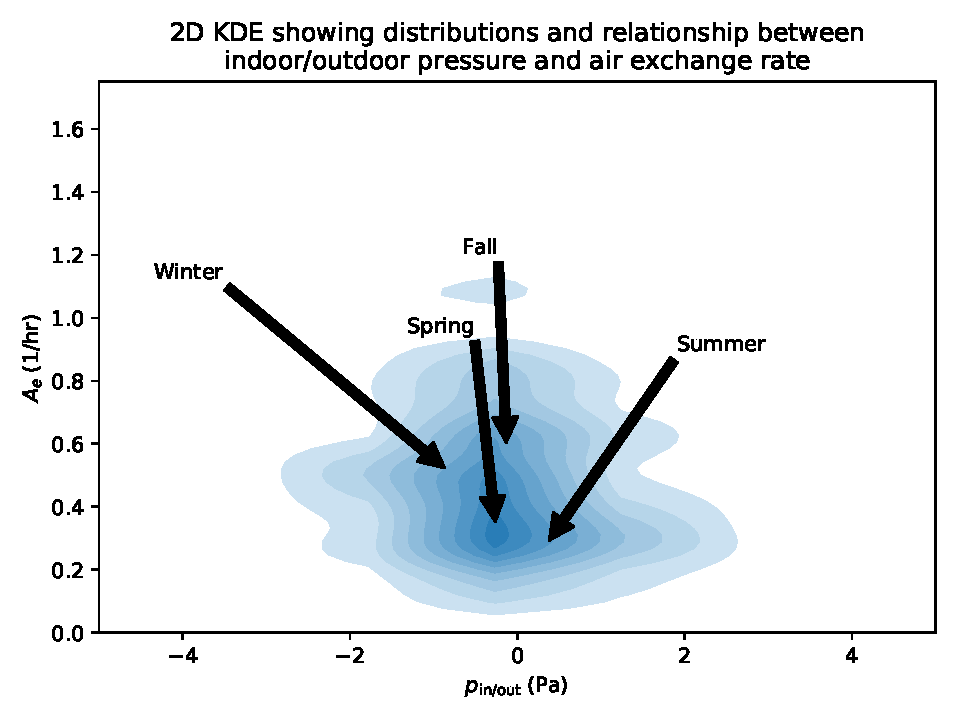
\includegraphics[width=\textwidth]{pressure_air_exchange_rate.pdf}
  \caption{Distributions of indoor pressurization and air exchange rate and their relationships; seasonal medians indicated by arrows.}
  \label{fig:pressure_air_exchange_rate_kde}
\end{figure}

\paragraph{Building Leakage Curves}

It is possible to quantify air exchange rate if a building is sufficiently pressurized through building leakage curves.
% TODO: Elaborate more on this once you've actually read something...

\subsection{Quantifying Pressure Difference Induction}\label{sec:quantifying_pressure}

% TODO: Write some short introduction here.

\paragraph{Wind Effects}

As the wind strikes a surface its velocity falls to zero, and the change in momentum is directly proportional to the change in pressure:
\begin{equation}\label{eq:wind_pressure_uncorrected}
  \Delta P = \frac{1}{2} \rho_\mathrm{air} u_\mathrm{wind}^2
\end{equation}
where $\Delta P$ is the change in pressure; $\rho_\mathrm{air}$ is the air density; and $u_\mathrm{wind}$ is the wind speed.\par

In reality however, the pressure drop is not quite so straightforward due to several factors, e.g. building envelope contains various structures and may be shielded by other objects.
To account for this, a drag or pressure coefficient $C_d$ is introduce to moderate the pressure drop:
\begin{equation}\label{eq:wind_pressure}
  \Delta P = C_d \frac{1}{2} \rho_\mathrm{air} u_\mathrm{wind}^2
\end{equation}
This coefficient is usually determined empirically from e.g. wind tunnel studies.

\paragraph{Temperature Effects}

The pressure of any fluid under the influence of gravity varies with elevation and the density of the fluid determines the magnitude of this pressure.
Air is a compressible fluid and its density depends on its temperature.
Therefore, if you separate two air masses between a wall, with each at a difference temperature, a pressure difference across the wall be induced, i.e. the \textit{stack effect}.

Assuming the ideal gas law applies and that the temperature on either side is constant then
\begin{equation}
  P = P_0 \exp{\Big( \frac{-M_\mathrm{air}gz}{RT} \Big)}
\end{equation}
determines the pressure variation across the wall.
Where $P$ is the pressure; $P_0$ the reference pressure ($z=0$); $M_\mathrm{air}$ is the molar weight of air; $z$ is the elevation; $g$ is the acceleration due to gravity; $R$ is the gas constant; and $T$ is the temperature.\par

This can be further simplified by defining $z_0$ which is the height at which the pressure on both sides of the wall are equal, i.e. $P_0$.
The pressure variation on either side can now be expressed in terms of distance from $z_0$, $z-z_0$.
Assuming that the interior and exterior has a constant temperature of $T_i$ and $T_o$ respectively, the difference in pressure between the two sides along the wall is
\begin{equation}
  \Delta P = P_0 \Big[ \exp{\Big( \frac{-M_\mathrm{air}g(z-z_0)}{RT_i} \Big)} - \exp{\Big( \frac{-M_\mathrm{air}g(z-z_0)}{RT_o} \Big)} \Big]
\end{equation}
Using that $e^{-x} = 1 - x$ for $x \ll 1$ the pressure difference can be expressed as
\begin{equation}
  \Delta P = \alpha \Big( \frac{1}{T_o} - \frac{1}{T_i} (z-z_0)\Big)
\end{equation}
where $\alpha = \frac{P_0 M_\mathrm{air} g}{R} \approx 3454 \; \mathrm{ \frac{Pa \cdot K}{m}Pa}$.
Here a negative pressure differnece, $\Delta P < 0$, indicates an inward flow.\par

% TODO: Write about other pressure generating sources too... not sure if there is any mathematics to describe this.
\paragraph{Other Effects}

Other factors also contribute to the pressure difference between the interior and exterior.
Some examples of these are various combustion processes (fireplaces), ventilation fans, or even human factors such as opening and closing doors or windows.

\subsection{Indoor Sources}

There are two types of indoor sources in VI.
The first are various products and items that contain the contaminant of concern and continuously emit these.
Some examples of these may be various cleaning products, degreasers, gasoline tanks, or even recently dry-cleaned clothing.
These are usually not considered to be part of the VI phenomena themselves (even though they can pose health risks) but rather items that need to be removed in a VI investigation to prevent false positives.\par

The second type are the walls, furniture, objects, or features inside the interior that sorb the contaminant vapors.
While these are not \textit{sources} in the strict sense, they may never the less contribute to the overall contaminant exposure.
How significant these secondary types of indoor sources are largely depend on the material.
Some, such as cinderblock concrete have a very large capacity to hold contaminant vapors while others such as fabrics do not.\par

% TODO: Add modeling about the first type of indoor sources here?

\paragraph{Sorption Processes}

Modeling the secondary type indoor sources (sorption onto materials) can be done with a simple equilibrium reaction:
\begin{equation}\label{eq:sorption_rxn}
  \mathrm{c^*} \underset{k_2}{\stackrel{k_1}{\rightleftharpoons}} \mathrm{c_{in}}
\end{equation}

% TODO: Finish this when you've progressed more with the paper
